\subsection{Maximum Likelihood estimation: non-compressive case}\label{sec:max-like}

Consider a received signal \(y \in \re^n\), composed of a deterministic signal \(\bar{s} \in \re^n\) corrupted by noise \(n \in \re^n\) (assumed to have zero mean and unit variance), i.e.

\begin{equation}
y = s + n
\end{equation}

We assume \(s\left(\Theta\right)\) comes from a fixed class of signals, with parameters indexed by a set \(\Theta\). For example

\begin{itemize}
\item The signal \(s\) is composed of a single frequency with unit amplitude \(s = e^{i \omega_0 k}\). In this case \( \Theta = \{\omega_j\}_{j=1}^n \) is the set of possible frequencies the signal may take on.

\item The signal \(s\) is a scaled and shifted version of a model signal \(f\): \(s(t) = Cf\left(t - \tau\right)\). In this case \(\Theta = \left(C, \tau \right)\).

\item The signal \(s\) can be expanded in some orthonormal basis, and that we have access to the basis functions \(\{\phi_i\}_{i=1}^n\):
\begin{equation}
s = \sum_{i=1}^n \alpha_i \phi_i
\end{equation}

In this case \(\Theta = \{\alpha_i, \phi_i\}_{i=1}^n\)

\end{itemize}

We can write the likelihood for \(y\) down as, for a given \(\Theta\), \(s\) is deterministic. Therefore y is a Gaussian random variable with mean \(s\):

\begin{equation}
f\left(y \mid s\right) = \left(\frac{1}{\sqrt{2\pi}} \right)^n \exp{\left( - \frac{\left(y-s(\Theta)\right)^T\left(y-s(\Theta)\right)}{2} \right)}
\end{equation}

Maximising this is equivalent to maximising:

\begin{equation}
\ln f\left(\Theta\right) = -\vectornorm{y}_2^2 + 2\langle y, s\left(\Theta\right)\rangle - \vectornorm{s}_2^2
\end{equation}

Since the terms \(\vectornorm{y}_2^2\) and \(\vectornorm{s}_2^2\) do not change, we can write the ML estimate of \(\Theta\) as:

\begin{equation}
\hat{\Theta} = \argmax_{\Theta} \langle y, s\left(\Theta\right)\rangle
\end{equation}

So, for example:

\begin{itemize}
\item If we receive a single tone corrupted by noise \(y = e^{i \omega_0 k} + n\) then we can estimate \(\omega_0\) by calculating \(\argmax_{\omega_i} \langle y, e^{i \omega_j k}\rangle = e^{i \omega_0 k}\) as the functions \(e^{i \omega_0 j k }\) are orthonormal: \(\langle e^{i \omega_l k}, e^{i \omega_r k} \rangle = \delta_{lr}\).

\item If we receive a signal composed of a sum of orthonormal basis functions we can estimate the coefficients \(\alpha_i\) as:

\begin{align}
\langle y, \phi_i\rangle\ =& \sum_{j=1}^n \alpha_j \phi_j^T\phi_i + n^T\phi_i \\
=& \alpha_i + \varepsilon_i
\end{align}

where \(\varepsilon_i = \langle n^T, \phi_i \rangle \) is some small error. Thus the maximum likelihood estimate of \(s\) is:

\begin{equation}
\hat{s} = \sum_{i=1}^n \hat{\alpha}_i \phi_i
\end{equation}

where

\begin{equation}
\hat{\alpha} = \langle y, \phi_i \rangle
\end{equation}

\end{itemize}

\begin{figure*}[h]
\centering
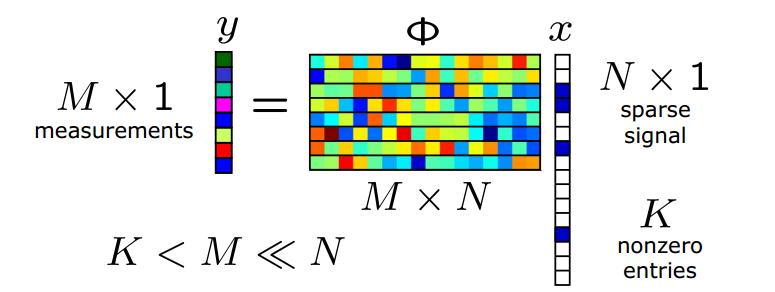
\includegraphics[height = 7 cm, width=\textwidth]{compressive_sensing_example.jpg}
\caption{A visualisation of the Compressive Sensing problem as an under-determined system}
\label{l1l2}
\end{figure*}


\begin{figure*}[h]
\centering
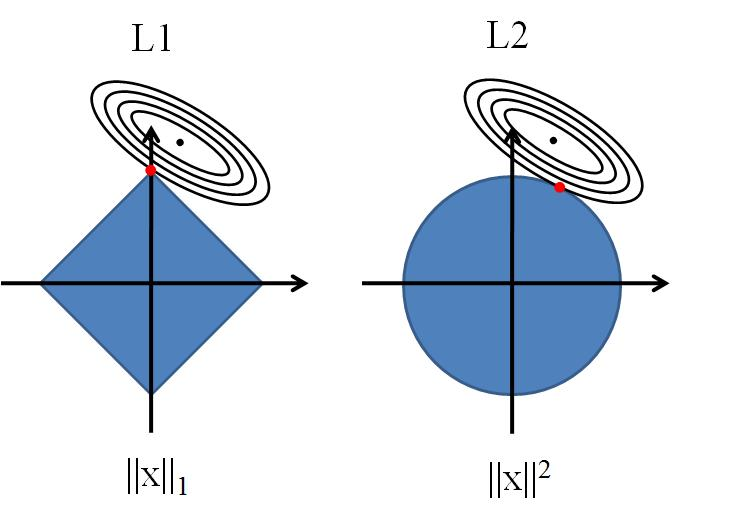
\includegraphics[height = 7 cm]{l1l2.jpg}
\caption{Solutions to the Compressive Sensing optimisation problem intersect the \(l_1\) norm the points where all components (but one) of the vector are zero (i.e. it is sparsity promoting) \cite{Tibshirani1996}}
\label{l1l2}
\end{figure*}
